\documentclass[a4paper,10pt]{article}
\usepackage[utf8]{inputenc}
 
% Blank line between paragraphs instead of indenting the first line
\usepackage{parskip}
\setlength{\parskip}{\baselineskip}

% Squash a bit more text onto a page
\usepackage{geometry}
\geometry{verbose,tmargin=15mm,bmargin=15mm,lmargin=15mm,rmargin=15mm}

\usepackage{graphicx}
\usepackage{listings}
\usepackage{amsmath}
\usepackage{verbatim}
\usepackage{color}
\usepackage{wrapfig}

% Indent verbatim environments
\makeatletter \def\verbatim@processline{\hspace*{2em}\the\verbatim@line\par}\makeatother

\definecolor{mygreen}{rgb}{0,0.6,0}
\definecolor{mygray}{rgb}{0.5,0.5,0.5}
\definecolor{mymauve}{rgb}{0.58,0,0.82}

\lstset { 
  backgroundcolor=\color{white},   % choose the background color; you must add \usepackage{color} or \usepackage{xcolor}
  basicstyle=\footnotesize,        % the size of the fonts that are used for the code
  breakatwhitespace=false,         % sets if automatic breaks should only happen at whitespace
  breaklines=true,                 % sets automatic line breaking
  captionpos=b,                    % sets the caption-position to bottom
  commentstyle=\color{mygreen},    % comment style
  deletekeywords={...},            % if you want to delete keywords from the given language
  escapeinside={\%*}{*)},          % if you want to add LaTeX within your code
  extendedchars=true,              % lets you use non-ASCII characters; for 8-bits encodings only, does not work with UTF-8
  frame=single,                    % adds a frame around the code
  keepspaces=true,                 % keeps spaces in text, useful for keeping indentation of code (possibly needs columns=flexible)
  keywordstyle=\color{blue},       % keyword style
  language=C++,                    % the language of the code
  morekeywords={*,DEVICES,
  				CONNECTIONS,
  				MONITORS,
  				END}, 	           % if you want to add more keywords to the set
  numbers=left,                    % where to put the line-numbers; possible values are (none, left, right)
  numbersep=5pt,                   % how far the line-numbers are from the code
  numberstyle=\tiny\color{mygray}, % the style that is used for the line-numbers
  rulecolor=\color{black},         % if not set, the frame-color may be changed on line-breaks within not-black text (e.g. comments (green here))
  showspaces=false,                % show spaces everywhere adding particular underscores; it overrides 'showstringspaces'
  showstringspaces=false,          % underline spaces within strings only
  showtabs=false,                  % show tabs within strings adding particular underscores
  stepnumber=1,                    % the step between two line-numbers. If it's 1, each line will be numbered
  stringstyle=\color{mymauve},     % string literal style
  tabsize=2,                       % sets default tabsize to 2 spaces
  title=\lstname                   % show the filename of files included with \lstinputlisting; also try caption instead of title
}

\begin{document}

\begin{center}
\LARGE \textbf{IIA GF2 Software: 2nd Interim Report}

\small Tim Hillel (th389) - Team 8
\end{center}

\section{Code Listings}
\subsection{Parser Class}
\subsubsection{parser.h}
\lstinputlisting[caption=parser.h]{../../src/parser.h}
\subsubsection{parser.cc}
\lstinputlisting[caption=parser.cc]{../../src/parser.cc}

I was mainly responsible for \texttt{parser.cc}, with input from Jamie Magee on the \texttt{connectionList} and \texttt{monitorList} functions. (Final ratio was around 75\% my work, 25\% his work.) 

\subsection{Error Class}
\subsubsection{error.h}
\lstinputlisting[caption=error.h]{../../src/error.h}
\subsubsection{error.cc}
\lstinputlisting[caption=error.cc]{../../src/error.cc}

\section{Test Definition Files}

\subsection{XOR Gate}
\subsubsection{Definition File}
\lstinputlisting[caption=xor.gf2]{../../examples/xor.gf2}
\subsubsection{Circuit Diagram}
\begin{figure}[h]
 \centering
 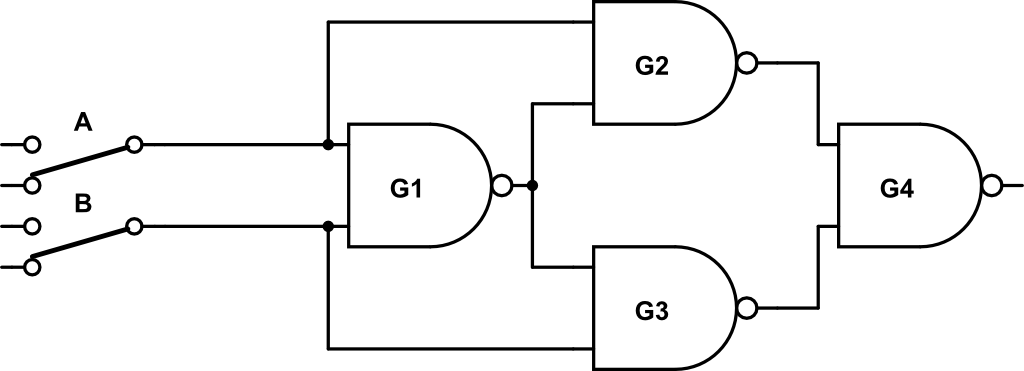
\includegraphics[width=8cm]{../../examples/xor.png}
 \caption{Circuit diagram of an XOR gate implemented using NAND gates}
 \label{fig:example-xor}
\end{figure}

\subsection{4-bit Adder}
\subsubsection{Definition File}
\lstinputlisting[caption=4bitadder.gf2]{../../examples/4bitadder.gf2}
\subsubsection{Circuit Diagram}
\begin{figure}[h]
 \centering
 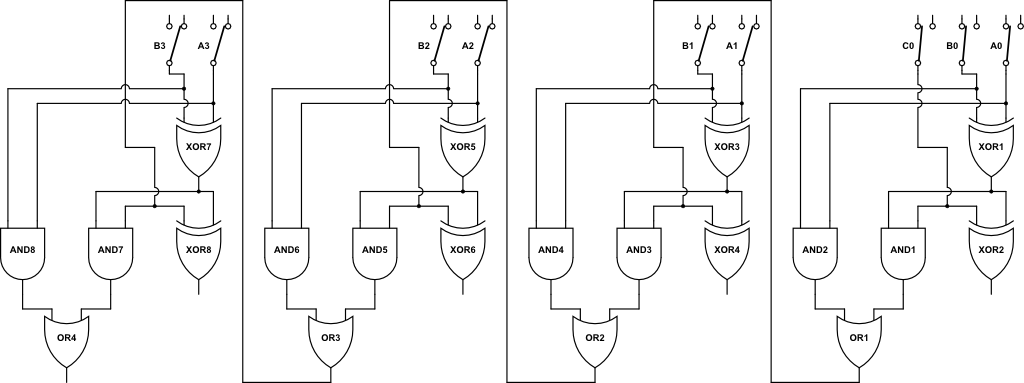
\includegraphics[width=16cm]{../../examples/4-bit-adder.png}
 \caption{Circuit diagram of a 4-bit adder}
 \label{fig:example-adder}
\end{figure}

\subsection{Serial In Parallel Out Shift Register}
\subsubsection{Definition File}
\lstinputlisting[caption=sipo.gf2]{../../examples/sipo.gf2}
\subsubsection{Circuit Diagram}

\begin{figure}[h]
 \centering
 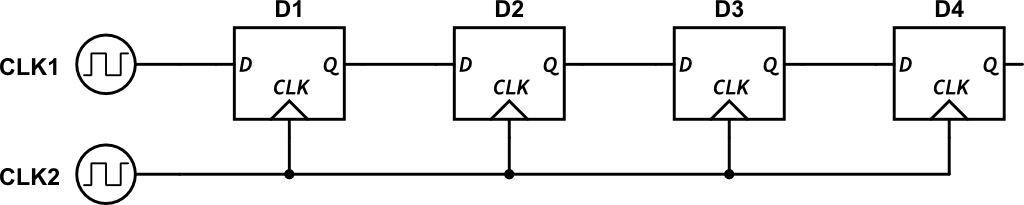
\includegraphics[width=12cm]{../../examples/sipo.png}
 \caption{Circuit diagram of a serial in parallel out shift register}
 \label{fig:example-sipo}
\end{figure}

\textbf{NB} The software used to draw the circuit diagram does not support the same style of D flip-flop used in the definition file, and Fig. \ref{fig:example-sipo} was the closest achievable.

\subsection{Gated D Latch}
\subsubsection{Definition File}
\lstinputlisting[caption=sipo.gf2]{../../examples/gateddlatch.gf2}
\subsubsection{Circuit Diagram}
\begin{figure}[h]
 \centering
 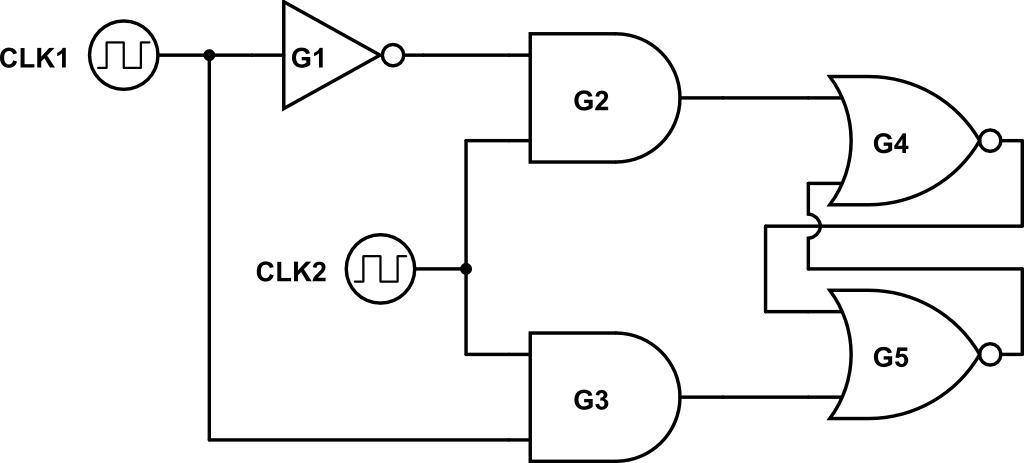
\includegraphics[width=12cm]{../../examples/gated-d-latch.png}
 \caption{Circuit diagram of a Gated D Latch}
 \label{fig:example-dlatch}
\end{figure}

\textbf{NB} The software used to draw the circuit diagram does not support the NAND gates with one input. Therefore the NAND gate G1 was substituted for a NOT gate as can be seen in Fig. \ref{fig:example-dlatch}.

\pagebreak

\section{User Guide}

To start the logic simulator, open a terminal window and browse to the \texttt{src} folder. Start the application by typing \texttt{./logsim} followed by the return key. You will then be presented with the default view.

\begin{figure}[h]
 \centering
 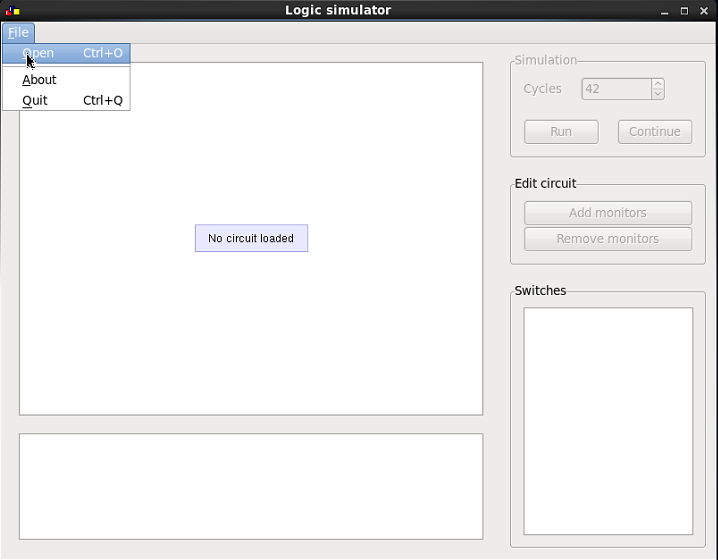
\includegraphics[width=.4\textwidth]{default}
 \caption{The default view upon opening the Logic Simulator}
 \label{fig:default}
\end{figure}

To open a definition file, click the \texttt{File} menu followed by the \texttt{Open} option. You will be presented with a file selection dialogue. The file selection dialogue will only show definition files (Files with the \texttt{.gf2} file extension). Upon selecting a file, any errors in the definition file will be written to the message window, otherwise the Logic Simulator is ready to use. 

In order to run a simulation you must first enter a number of cycles you wish the simulation to run for (default is \texttt{42}) then press the run button. The monitored signals will be displayed in the left display panel. You may choose to continue the simulation by pressing the continue button.

\begin{figure}[h]
 \centering
 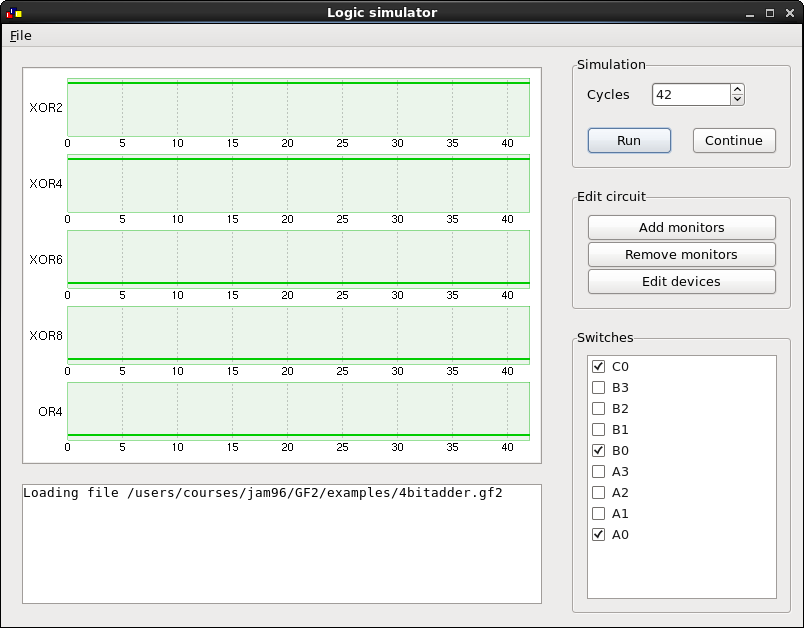
\includegraphics[width=.4\textwidth]{simulation}
 \caption{The  view upon running a simulation}
 \label{fig:default}
\end{figure}

\begin{wrapfigure}{l}{0.5\textwidth}
  \begin{center}
    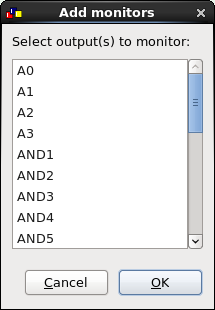
\includegraphics[width=0.2\textwidth]{monitors}
  \end{center}
  \caption{Add monitors dialogue}
\end{wrapfigure}

You can also edit the monitors from within the logic simulator. To add monitors, click the \texttt{Add monitors} button and select the monitor, or monitors, you wish to add followed by the \texttt{OK} button. To remove monitors, press the \texttt{Remove monitors} button and select the monitor, or monitors, you wish to remove followed by the \texttt{OK} button

In addition, if your circuit contains any  switches, you can change the state of the switch by changing the state of the check box beside its name.

\end{document}
